
\begin{figure}[htbp]
\centering
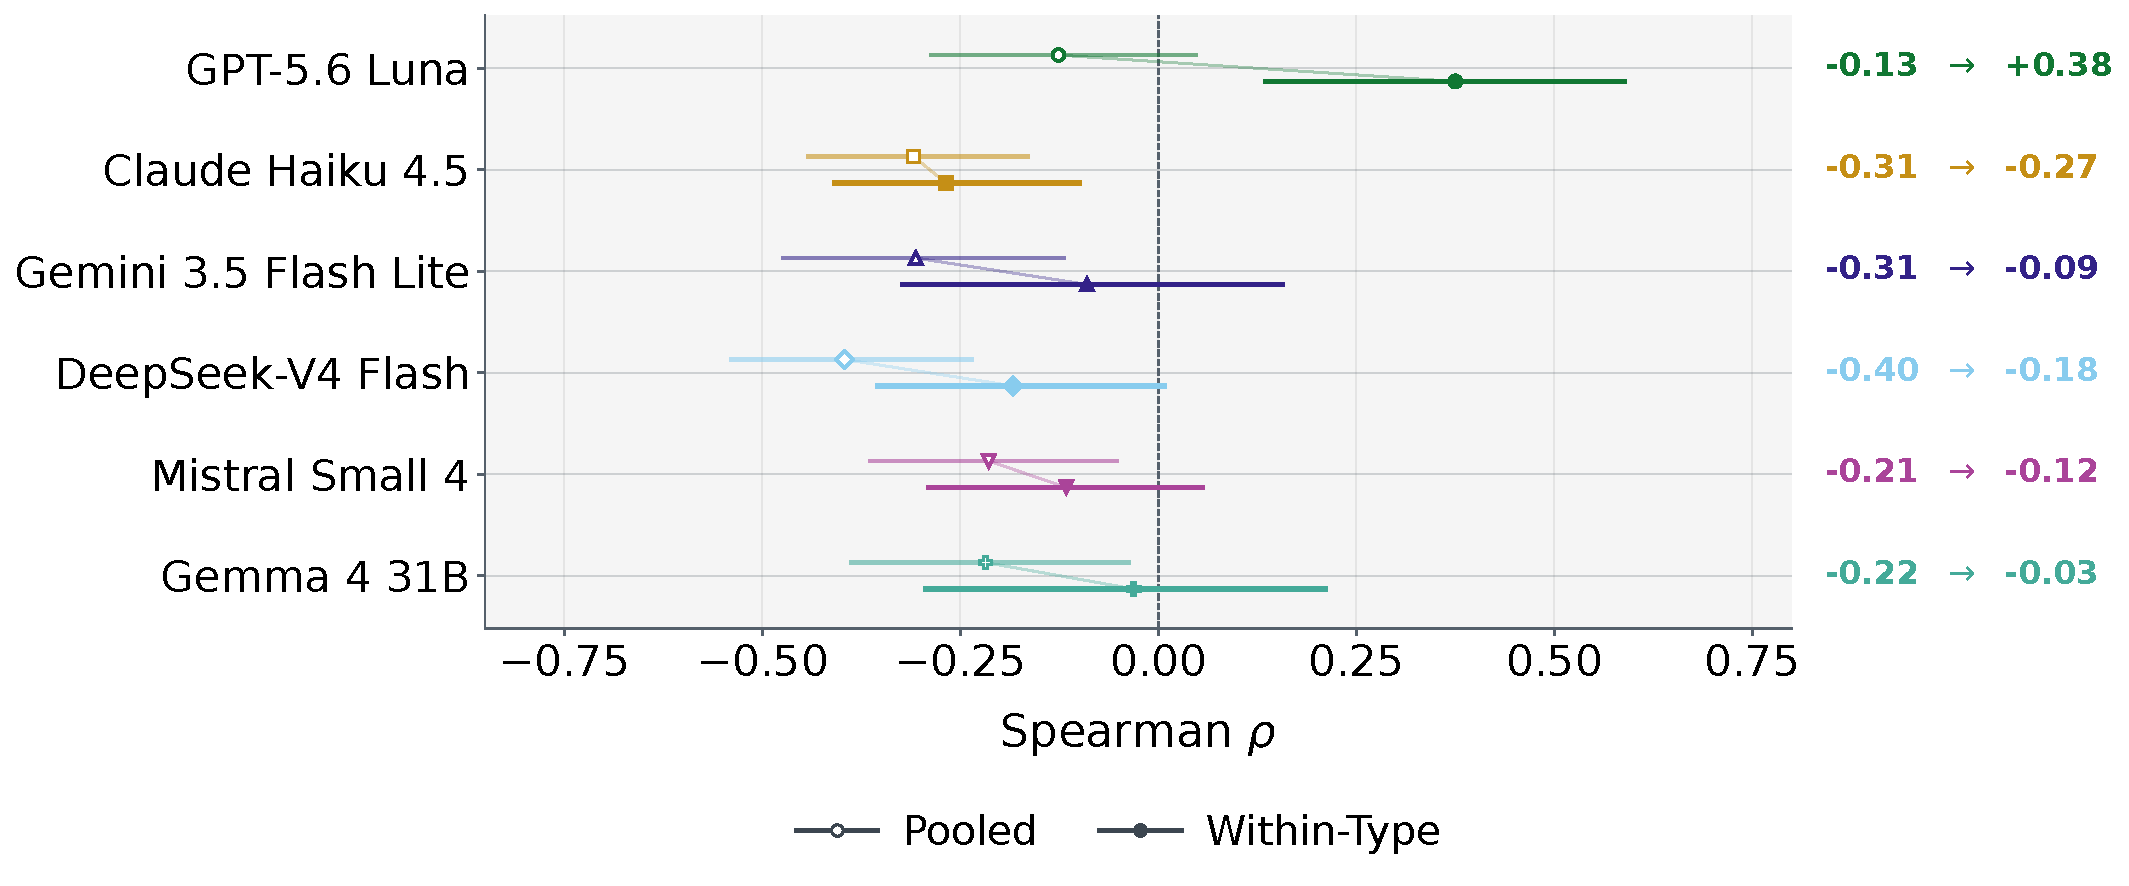
\includegraphics[width=0.8\textwidth]{joint/joint_association.pdf}
\caption{\emph{Experiment 1} $\vert$ Concordance Coefficient by Model}
\label{fig:joint-association}
\vspace{0.4em}
\begin{minipage}{\textwidth}
\footnotesize
\emph{Note.} Spearman correlation between the two age effects at scenario level,
by scenario type. A positive coefficient is a model that simplifies most where it
also refuses most. The pooled coefficient is drawn for reference but is not
comparable, since it mixes types. Benign carries none, its refusal shift being
constant, and neither does Rights on GPT-5.6 Luna, which refuses nothing there.
Conditioning on type leaves four models weakened, Claude Haiku 4.5 negative and
GPT-5.6 Luna reversed, so the two age effects are not reliably linked.
\end{minipage}
\end{figure}
